\documentclass[14pt]{extarticle}
\usepackage[left=15mm, top=15mm, right=20mm, bottom=15mm, nohead, footskip=10mm]{geometry}
\usepackage[T2A]{fontenc}
\usepackage[english, russian]{babel} % Языки: русский, английский
\usepackage[utf8]{inputenc}
\usepackage{graphicx}
\usepackage{amsmath}
\usepackage{animate}
\usepackage{color} %% это для отображения цвета в коде
\usepackage{listings} %% собственно, это и есть пакет listings
\usepackage{subcaption}
\usepackage{caption}
\DeclareCaptionFont{white}{\color{white}} %% это сделает текст заголовка белым
%% код ниже нарисует серую рамочку вокруг заголовка кода.
\DeclareCaptionFormat{listing}{\colorbox{gray}{\parbox{\textwidth}{#1#2#3}}}
\captionsetup[lstlisting]{format=listing,labelfont=white,textfont=white}

\lstset{ %
language=Java,                 % выбор языка для подсветки (здесь это С)
basicstyle=\small\sffamily, % размер и начертание шрифта для подсветки кода
numbers=left,               % где поставить нумерацию строк (слева\справа)
numberstyle=\tiny,           % размер шрифта для номеров строк
stepnumber=1,                   % размер шага между двумя номерами строк
numbersep=5pt,                % как далеко отстоят номера строк от подсвечиваемого кода
backgroundcolor=\color{white}, % цвет фона подсветки - используем \usepackage{color}
showspaces=false,            % показывать или нет пробелы специальными отступами
showstringspaces=false,      % показывать или нет пробелы в строках
showtabs=false,             % показывать или нет табуляцию в строках
frame=single,              % рисовать рамку вокруг кода
tabsize=2,                 % размер табуляции по умолчанию равен 2 пробелам
captionpos=t,              % позиция заголовка вверху [t] или внизу [b]
breaklines=true,           % автоматически переносить строки (да\нет)
breakatwhitespace=false, % переносить строки только если есть пробел
escapeinside={\%*}{*)}   % если нужно добавить комментарии в коде
}


\begin{document}

\begin{center}
\hfill \break
\large{Министерство науки и высшего образования Российской федерации}\\
\footnotesize{ФЕДЕРАЛЬНОЕ ГОСУДАРСТВЕННОЕ БЮДЖЕТНОЕ ОБРАЗОВАТЕЛЬНОЕ УЧРЕЖДЕНИЕ}\\
\footnotesize{ВЫСШЕГО ПРОФЕССИОНАЛЬНОГО ОБРАЗОВАНИЯ}\\
\small{\textbf{«АЛТАЙСКИЙ ГОСУДАРСТВЕННЫЙ УНИВЕРСИТЕТ»}}\\
\hfill \break
\normalsize{Институт цифровых технологий, электроники и физики}\\
 \hfill \break
\normalsize{Кафедра вычислительной техники и электроники}\\
\hfill\break
\hfill \break
\hfill \break
\hfill \break
\large{Курс <<Математическое моделирование>>\\ Отчет по лабораторной работе №3\\ <<Игра ``Жизнь''>>}\\
\end{center}
\hfill \break
\hfill \break
\hfill \break
\hfill \break
\hfill \break

\normalsize{
  \begin{flushright}
    \begin{tabular}{rcr}
      & Выполнил: & студент 585гр.\\\\
      & Роженцев А.К. &\underline{\hspace{3cm}}\\\\
      & Проверил: ст.пр.\\\\
      & Уланов П.Н. & \underline{\hspace{3cm}}
    \end{tabular}
  \end{flushright}
}
\hfill \break
\hfill \break
\hfill \break
\hfill \break
\hfill \break
\begin{center} Барнаул 2020 \end{center}
\thispagestyle{empty}
\newpage
\section{Цель работы}
Реализовать программу, моделирующую игру «Жизнь» с такими правилами:
\begin{itemize}
  \item Клетки на квадратной доске могут находиться в двух состояниях: «живое» и «мертвое».
  \item  «Живая» клетка выживает на очередном временном
шаге, если имеет только 2 или 3 живых соседа.
  \item Если соседей меньше двух, клетка умирает из-за обособленности, а если больше трех,
то из-за скученности (перенаселения).
  \item «Мертвая» оживает на очередном шаге только в том случае, если имеет 3 живых соседа.
  \item  У
каждой клетки 8 соседей: клетки, имеющие с ней общие стороны
или вершины.
\item Изменение состояния всех клеток происходит одновременно.

\end{itemize}

\section{Задание}

\begin{enumerate}
  \item Реализовать программу, моделирующую игру ``Жизнь''.
  \item Задать центральную часть поля случайной конфигурацией.
Размеры случайной области от 3х3 до 10х10.
  \item Многократными запусками программы найти начальные конфигурации, приводящие к:
  \begin{itemize}
    \item вымиранию
    \item стабильной конфигурации
    \item периодической конфигурации
    \item конфигурации, развивающийся не менее 100 поколений
  \end{itemize}


\end{enumerate}


\newpage
\section{Программа}

\begin{figure}[!h]
  \centering
  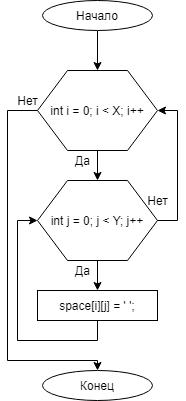
\includegraphics[width=0.45\textwidth]{initialization.png}
  \caption{Подпрограмма initialization}
\end{figure}
\newpage

\begin{figure}[!h]
  \centering
  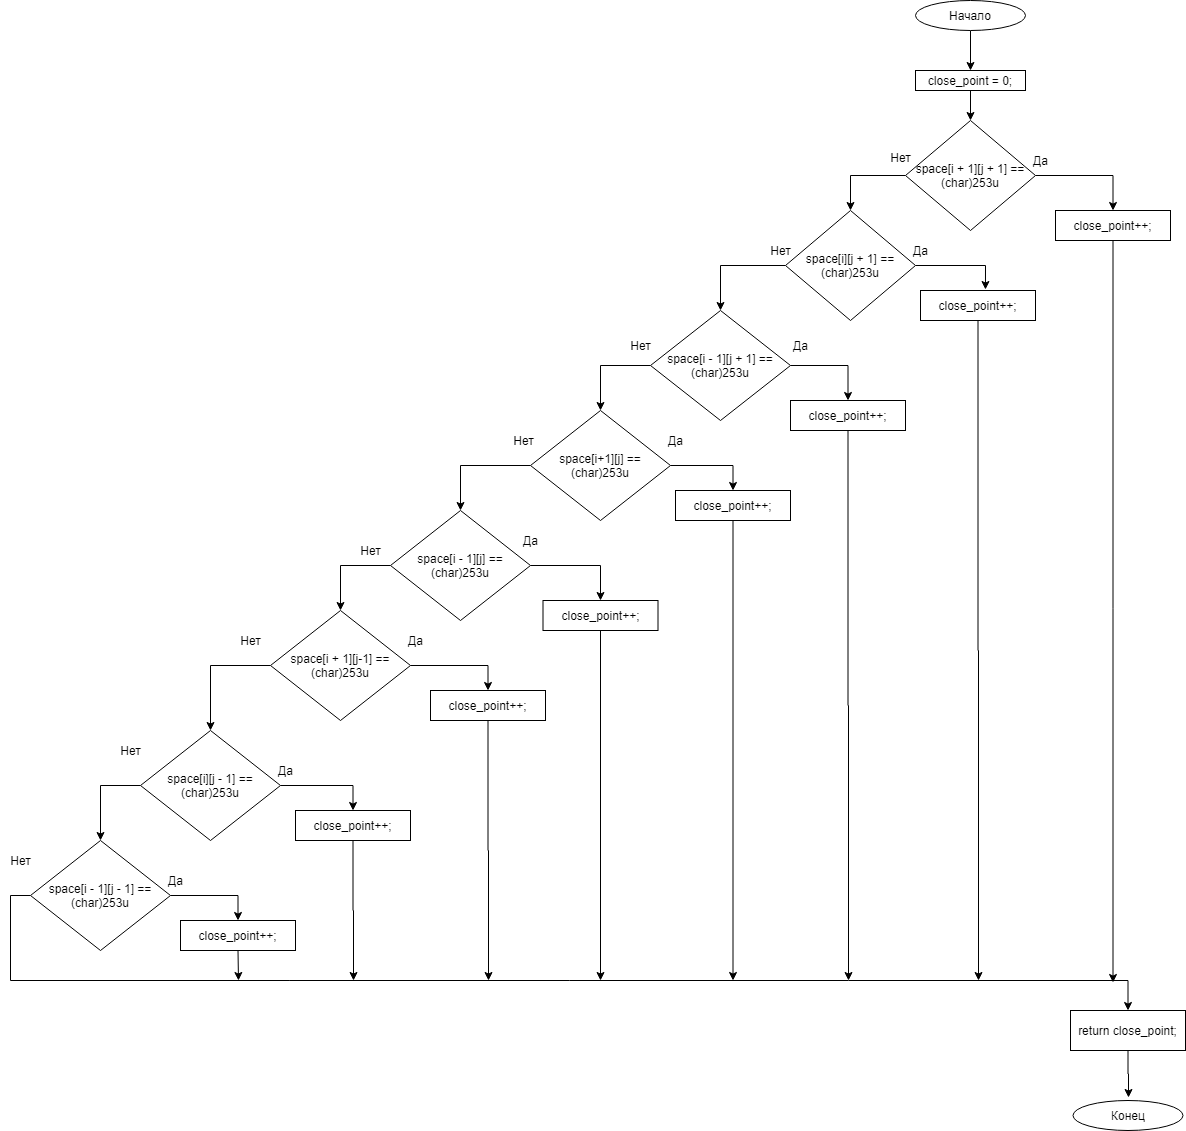
\includegraphics[width=1\textwidth]{FINS_POINTS.png}
  \caption{Подпрограмма FIND\_POINTS}
\end{figure}
\newpage

\begin{figure}[!h]
  \centering
  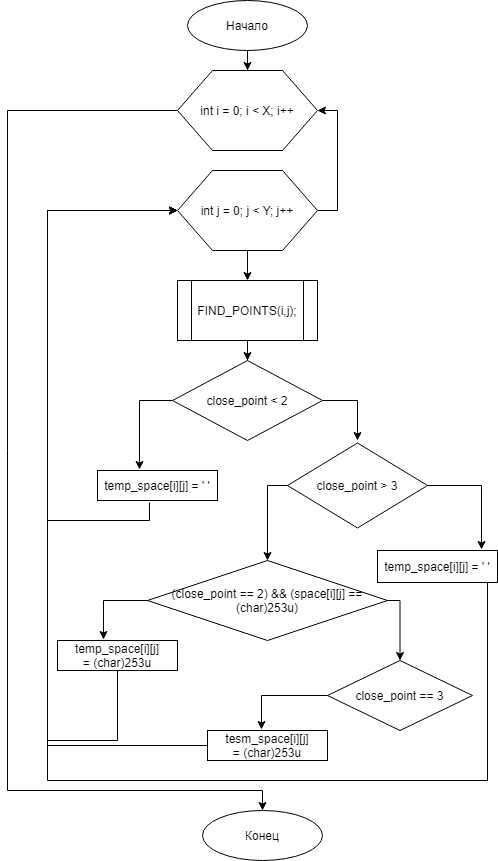
\includegraphics[width=0.5\textwidth  ]{RULES.png}
  \caption{Подпрограмма RULES}
\end{figure}
\newpage

\begin{figure}[!h]
  \centering
  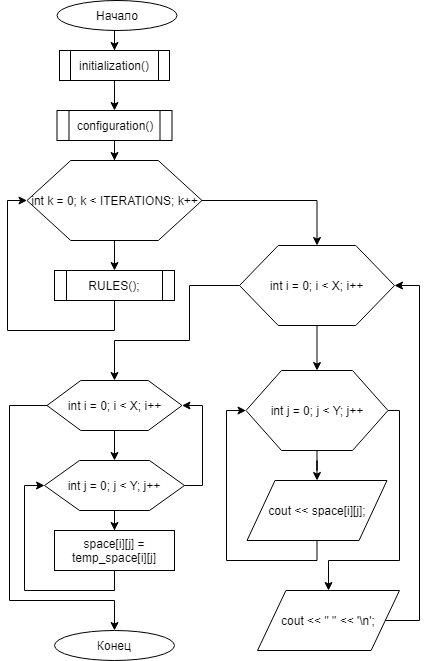
\includegraphics[width=0.5\textwidth]{main.png}
  \caption{Основная программа main}
\end{figure}
\newpage




\hfill \break
\section{Конфигурации}
\begin{figure}[!h]
  \centering
  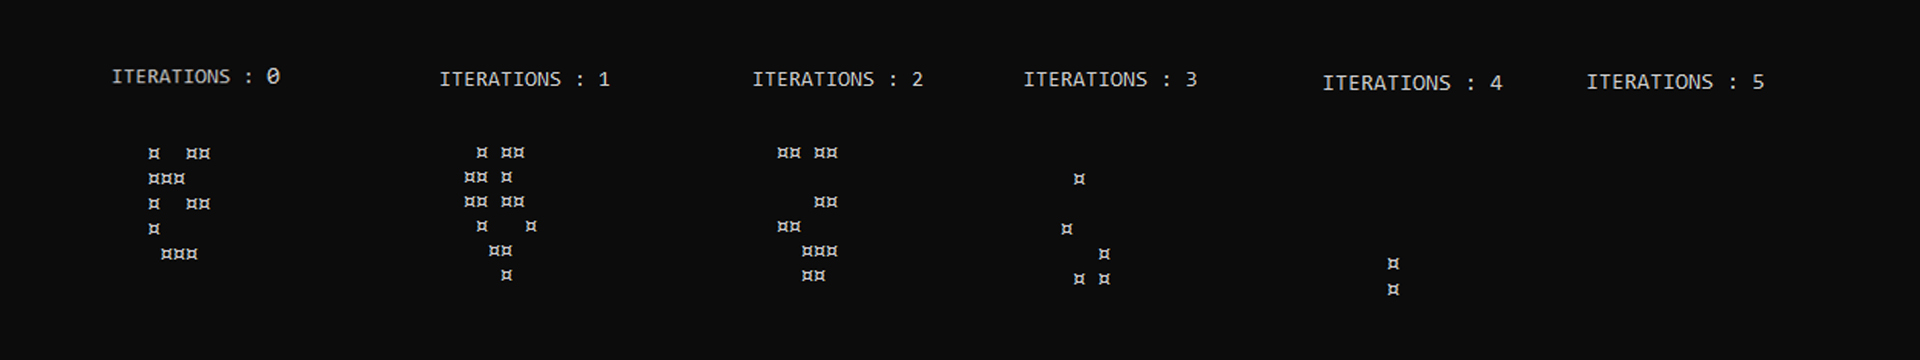
\includegraphics[width=1\textwidth]{vimiranie.jpg}
  \caption{Вымирание.}
\end{figure}

\begin{figure}[!h]
  \centering
  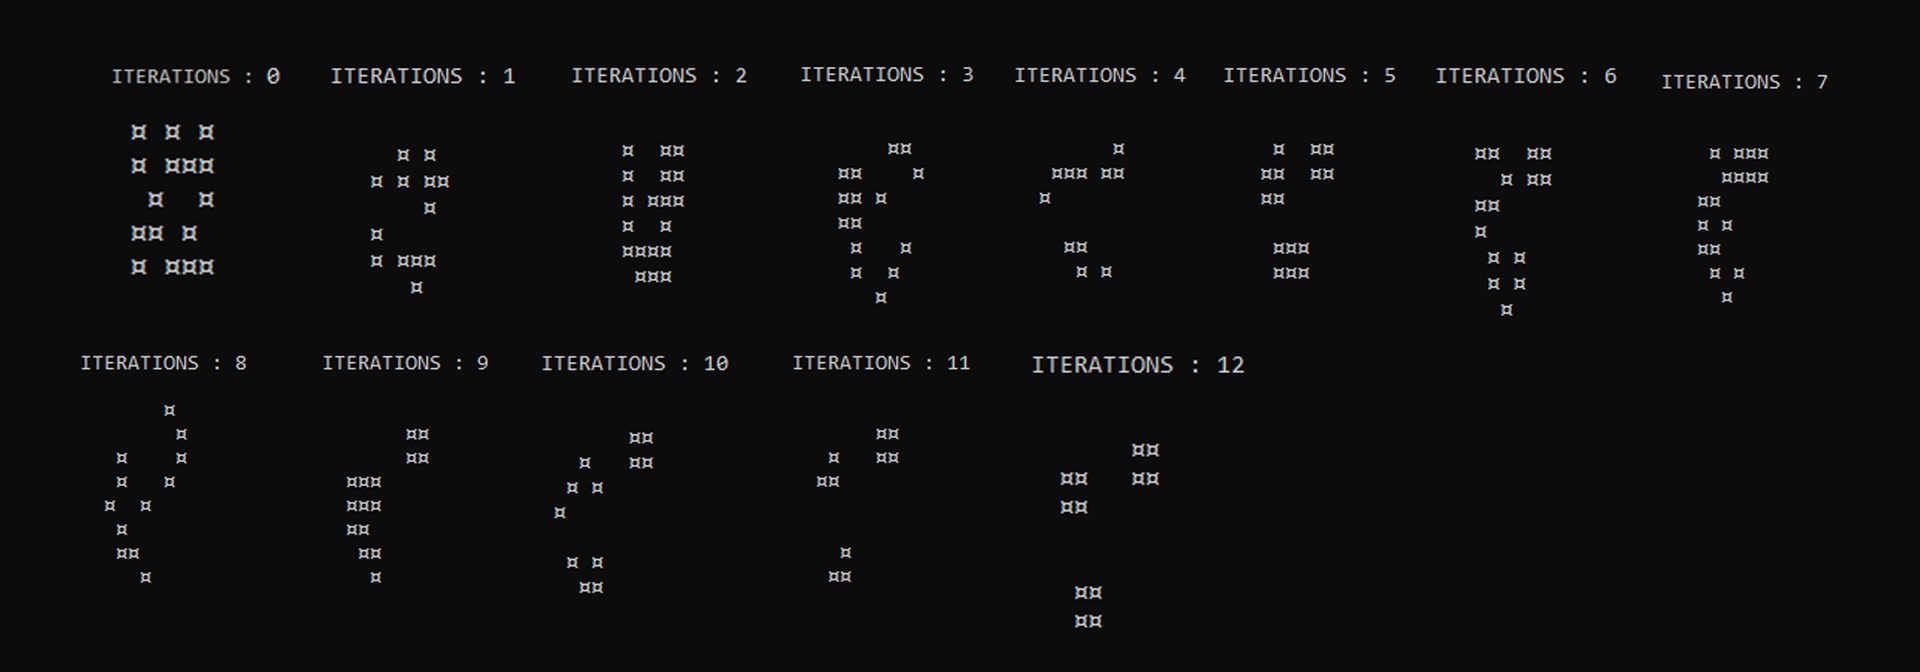
\includegraphics[width=1\textwidth]{stabilnost.jpg}
  \caption{Стабильная конфигурация.}
\end{figure}

\begin{figure}[!h]
  \centering
  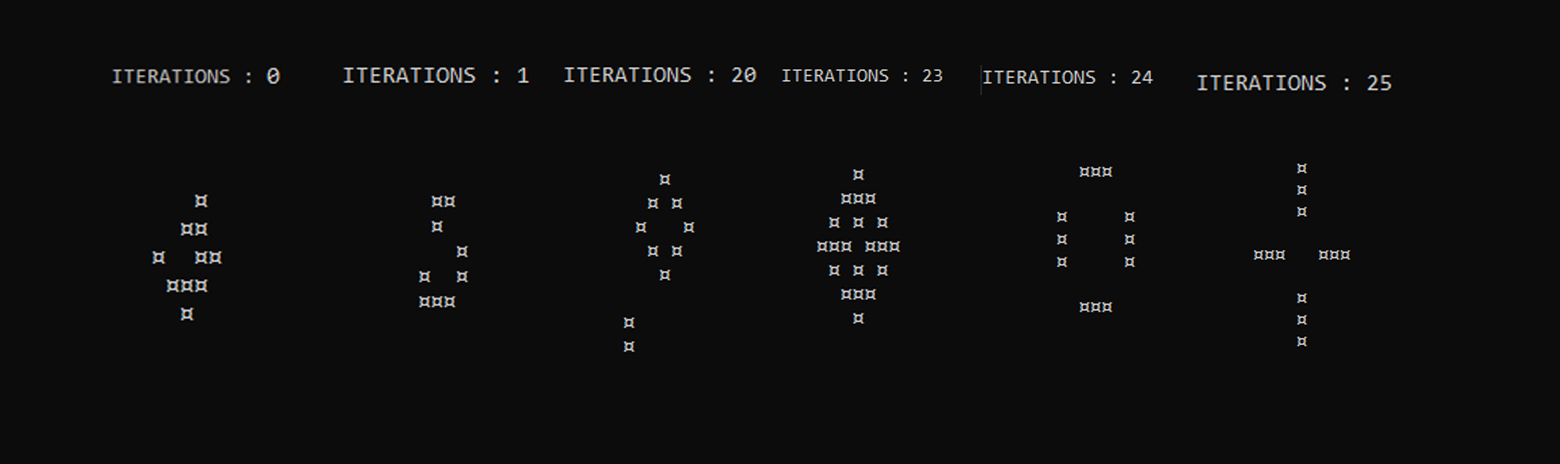
\includegraphics[width=1\textwidth]{PERIOD.jpg}
  \caption{Периодическая конфигурация.}
\end{figure}


\hfill \break

\newpage
\section{Код программы}

\begin{lstlisting}
#include <iostream>
#include <conio.h>
#include <stdio.h>
#include<Windows.h>
#include <stdlib.h>
#include <time.h> 


using namespace std;
#define ITERATIONS 1000
#define X 30 
#define Y 30

char space[X][Y];
char temp_space[X][Y];
int close_point;

void initialization(){
	for (int i = 0; i < X; i++) {
		for (int j = 0; j < Y; j++) {
			space[i][j] = ' ';
		}
	}
}

void configurations(){
	space[3][6] = (char)253u;
	space[4][5] = (char)253u;
	space[4][6] = (char)253u;
	space[5][3] = (char)253u;
	space[5][6] = (char)253u;
	space[5][7] = (char)253u;
	space[6][4] = (char)253u;
	space[6][5] = (char)253u;
	space[6][7] = (char)253u;
	space[7][5] = (char)253u;
}


int FIND_POINTS(int i, int j){
	close_point = 0;
	if (space[i + 1][j + 1] == (char)253u)
	{
		close_point++;
	}
	if (space[i][j + 1] == (char)253u)
	{
		close_point++;
	}
	if (space[i - 1][j + 1] == (char)253u)
	{
		close_point++;
	}
	if (space[i+1][j] == (char)253u)
	{
		close_point++;
	}
	if (space[i - 1][j] == (char)253u)
	{
		close_point++;
	}
	if (space[i + 1][j-1] == (char)253u)
	{
		close_point++;
	}
	if (space[i][j - 1] == (char)253u)
	{
		close_point++;
	}
	if (space[i - 1][j - 1] == (char)253u)
	{
		close_point++;
	}
	return close_point;
}

void RULES(){
	for (int i = 0; i < X; i++) {
		for (int j = 0; j < Y; j++) {
			FIND_POINTS(i,j);
			if (close_point < 2)
			{
				temp_space[i][j] = ' ';
			}
			else if (close_point > 3)
			{
				temp_space[i][j] = ' ';
			}
			else if ((close_point == 2) && (space[i][j] == (char)253u))
			{
				temp_space[i][j] = (char)253u;
			}
			else if (close_point == 3)
			{
				temp_space[i][j] = (char)253u;
			}
		}
	}
}

int main(){ 
	initialization();
	configurations();
	for (int k = 0; k < ITERATIONS; k++){
		RULES();
		for (int i = 0; i < X; i++) {
			for (int j = 0; j < Y; j++) {
				cout << space[i][j];
			}
			cout << " " << '\n';
		}
		for (int i = 0; i < X; i++) {
			for (int j = 0; j < Y; j++) {
				space[i][j] = temp_space[i][j];
			}
		}
		_getch();
		system("cls");
		cout<<"ITERATIONS : "<<k+1;
	}
	_getch();
}
\end{lstlisting}

\end{document}
